\documentclass[11pt,a4paper]{article}

\newcommand{\tumsoTime}{09:00 น. - 12:00 น.}
\newcommand{\tumsoRound}{1}

\usepackage{../tumso}

\begin{document}

\begin{problem}{Caeskh Enigma}{standard input}{standard output}{1 second}{64 megabytes}{300}

Caesar Cipher เป็นวิธีการเข้ารหัสข้อความที่หลาย ๆ คนคงรู้จักดี การเข้ารหัสข้อความแบบ Caesar Cipher นั้นง่ายมาก เพียงแค่แทนตัวอักษรแต่ละตัว ด้วยตัวอักษร 3 ตัวถัดไปในภาษาอังกฤษเท่านั้น ยกตัวอย่าง หากต้องการเข้ารหัสคำว่า \texttt{CAESAR} โดยกำหนดให้ $k=3$ ก็จะได้คำว่า \texttt{FDHVDU} ออกมา
\begin{center}
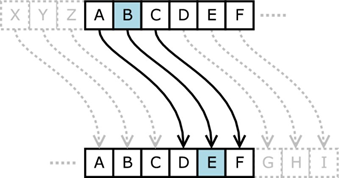
\includegraphics[width=10cm]{caesar.png}
\end{center}

Caeskh ไม่ชอบ Caesar Cipher เพราะมันง่ายเกินไป เขาจึงสร้างวิธีการเข้ารหัสแบบใหม่ขึ้นมาเอง ดังนี้

ก่อนอื่น Caeskh จะเขียนคำที่ต้องการเข้ารหัสเป็นตัวเลขโดยกำหนดให้ A = 1, B = 2, C = 3, ..., Z = 26 เช่น \texttt{CAESAR} ต้องเขียนเป็น \texttt{31519118} สังเกตว่านอกจาก \texttt{CAESAR} แล้วอาจจะมีคำอื่นที่สามารถแปลงเป็นเลข \texttt{31519118} ได้ เช่น \texttt{CAEAIKH}
\begin{center}
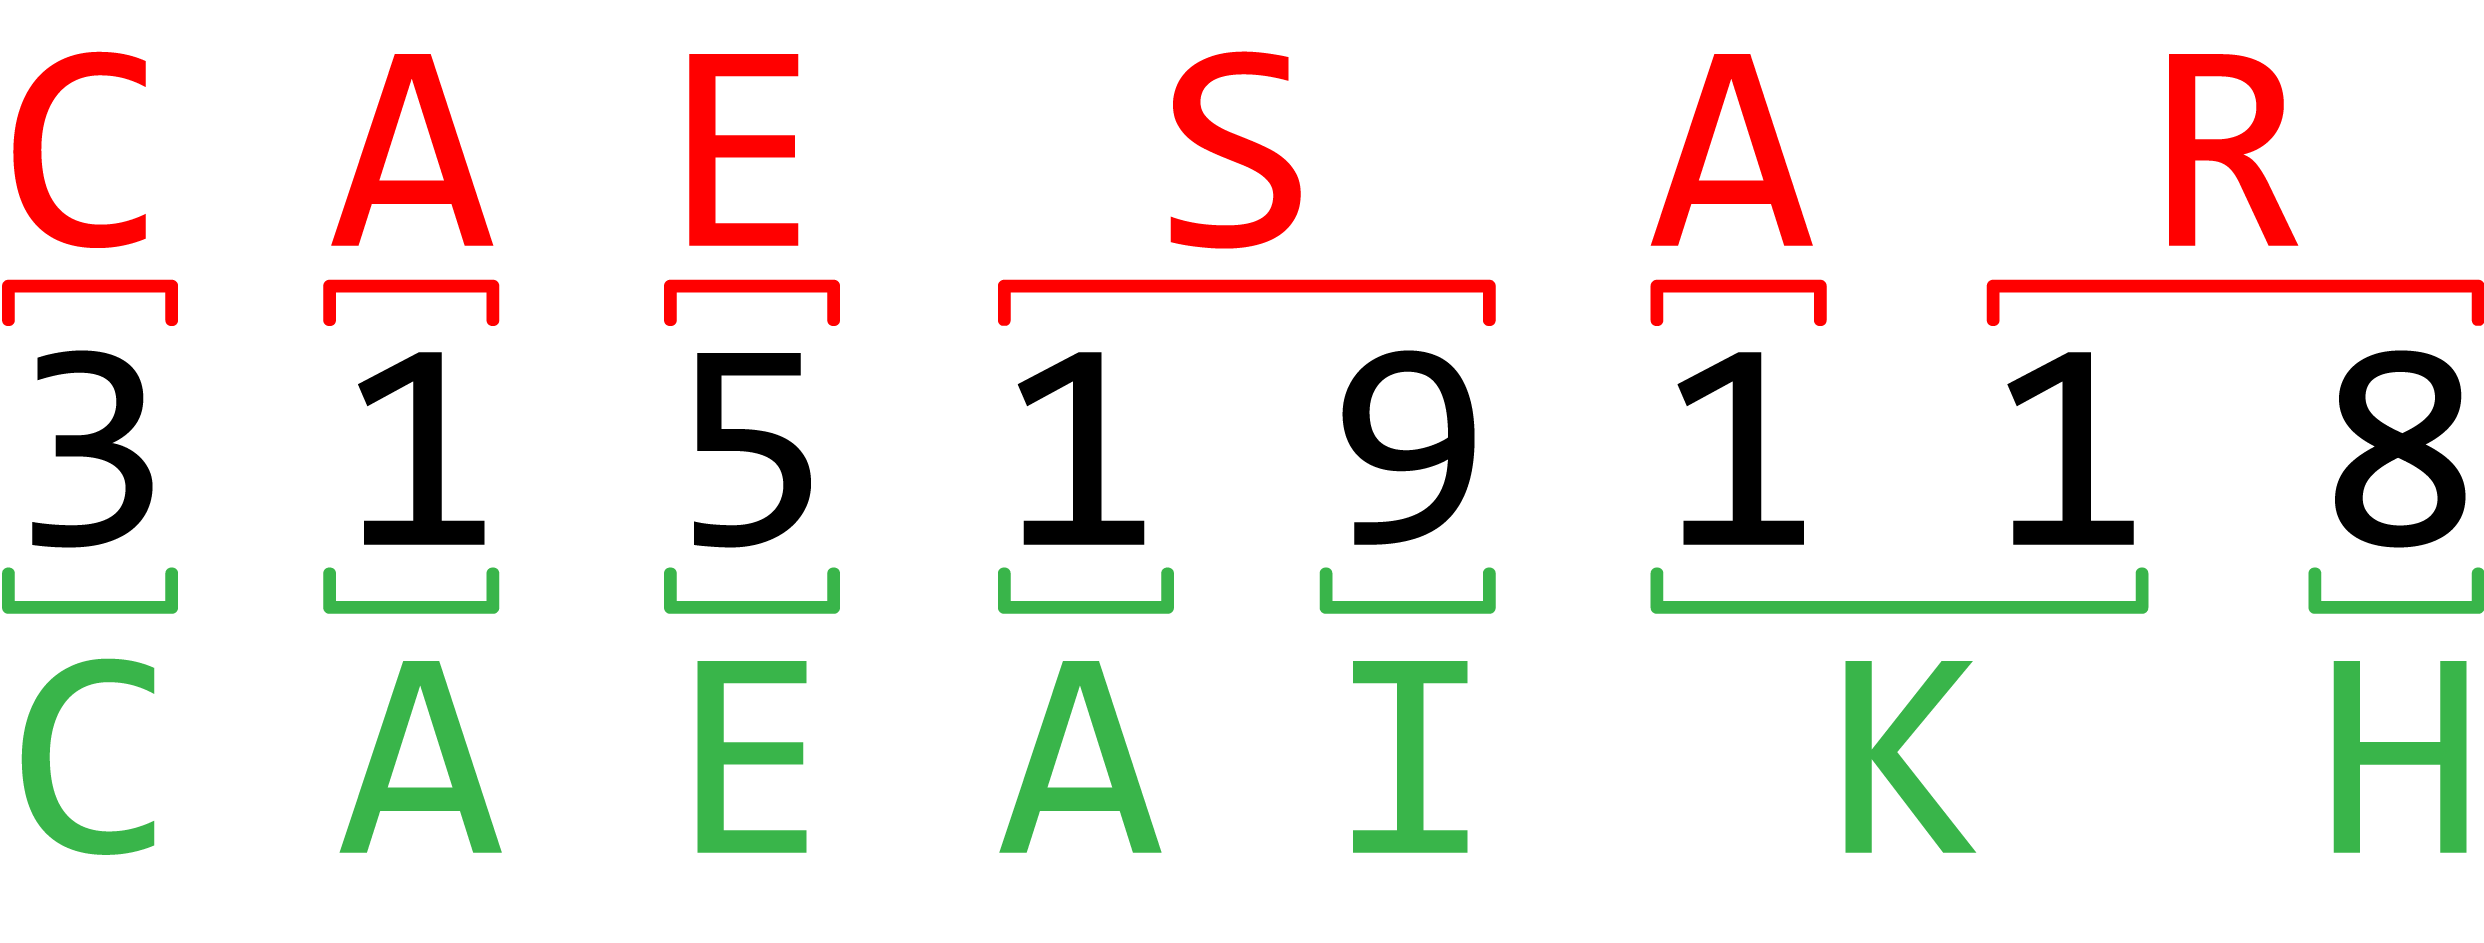
\includegraphics[width=10cm]{caeskh.png}
\end{center}

คำที่สามารถแปลงเป็นเลข \texttt{31519118} ทั้งหมดมีดังนี้:
1. \texttt{CAEAIAAH}
2. \texttt{CAEAIAR}
3. \texttt{CAEAIKH}
4. \texttt{CAESAAH}
5. \texttt{CAESAR}
6. \texttt{CAESKH}
7. \texttt{COAIAAH}
8. \texttt{COAIAR}
9. \texttt{COAIKH}
10. \texttt{COSAAH}
11. \texttt{COSAR}
12. \texttt{COSKH}

สังเกตว่า \texttt{CAESAR} เป็นคำที่ 5 ในรายการ นาย Caeskh จะเลือกคำในลำดับถัดไป โดยถือว่าคำนั้นเป็นคำที่เข้ารหัสแล้ว ในที่นี้จะได้คำว่า \texttt{CAESKH} ซึ่งเป็นคำที่ 6 พอดี

หน้าที่ของคุณคือหาว่า หากนำข้อความที่กำหนดให้มาเข้ารหัสตามวิธีที่ระบุไว้ข้างต้น จะได้ข้อความอะไร

\InputFile
ข้อมูลนำเข้ามีเพียงบรรทัดเดียว เป็นข้อความ $S$ ที่ประกอบด้วยตัวอักษรภาษาอังกฤษพิมพ์ใหญ่ ($1 \leq |S| \leq 10^5$)

\OutputFile
ตอบเพียงบรรทัดเดียว ข้อความ $S$ หลังเข้ารหัสแล้ว รับประกันว่าสามารถเข้ารหัสข้อความ $S$ ได้เสมอ ($S$ จะไม่อยู่ลำดับสุดท้ายหากเรียงตามพจนานุกรมตามที่กล่าวไว้ในโจทย์)

\Scoring
ชุดทดสอบจะถูกแบ่งเป็น 3 ชุด จะได้คะแนนในแต่ละชุดก็ต่อเมื่อโปรแกรมให้ผลลัพธ์ถูกต้องในชุดทดสอบย่อยทั้งหมด

\begin{description}

\item[ชุดที่ 1 (62 คะแนน)] จะมี $1 \leq |S| \leq 8$

\item[ชุดที่ 2 (98 คะแนน)] จะมี $1 \leq |S| \leq 50$

\item[ชุดที่ 3 (140 คะแนน)] ไม่มีเงื่อนไขเพิ่มเติมนอกเหนือจากที่ระบุไว้ในโจทย์

\end{description}

\Examples

\begin{example}
\exmpfile{example.01}{example.01.a}%
\end{example}

\end{problem}




\end{document}
